\documentclass[a4paper,12pt]{article}
\usepackage[UTF8]{ctex}
\usepackage{listings}
\lstset{
	breaklines,                                 % 自动将长的代码行换行排版
	extendedchars=false,                        % 解决代码跨页时,章节标题,页眉等汉字不显示的问题
	backgroundcolor=\color[rgb]{0.96,0.96,0.96},% 背景颜色
	keywordstyle=\color{blue}\bfseries,         % 关键字颜色
	identifierstyle=\color{black},              % 普通标识符颜色
	commentstyle=\color[rgb]{0,0.6,0},          % 注释颜色
	stringstyle=\color[rgb]{0.58,0,0.82},       % 字符串颜色
	showstringspaces=false,                     % 不显示字符串内的空格
	numbers=left,                               % 显示行号
	captionpos=t,                               % title在上方(在bottom即为b)
	frame=single,                               % 设置代码框形式
	rulecolor=\color[rgb]{0.8,0.8,0.8},         % 设置代码框颜色
}  



%\usepackage{xeCJK}
\usepackage{times}
\usepackage{setspace}
\usepackage{fancyhdr}
\usepackage{graphicx}
\usepackage{wrapfig}
\usepackage{array}  
\usepackage{fontspec,xunicode,xltxtra}
\usepackage{titlesec}
\usepackage{titletoc}
\usepackage[titletoc]{appendix}
\usepackage[top=30mm,bottom=30mm,left=20mm,right=20mm]{geometry}
\usepackage{cite}
\usepackage{listings}
\usepackage[hidelinks]{hyperref}
\usepackage{amsmath}
\usepackage[framed,numbered,autolinebreaks,useliterate]{mcode} % 插入代码
\XeTeXlinebreaklocale "zh"
\XeTeXlinebreakskip = 0pt plus 1pt minus 0.1pt



%---------------------------------------------------------------------
%	章节标题设置
%---------------------------------------------------------------------
\titleformat{\chapter}{\centering\zihao{-1}\heiti}{实验\chinese{chapter}}{1em}{}
\titlespacing{\chapter}{0pt}{*0}{*6}

%---------------------------------------------------------------------
%	摘要标题设置
%---------------------------------------------------------------------
\renewcommand{\abstractname}{\zihao{-3} 摘\quad 要}

%---------------------------------------------------------------------
%	参考文献设置
%---------------------------------------------------------------------
%\renewcommand{\bibname}{\zihao{2}{\hspace{\fill}参\hspace{0.5em}考\hspace{0.5em}文\hspace{0.5em}献\hspace{\fill}}}

%---------------------------------------------------------------------
%	引用文献设置为上标
%---------------------------------------------------------------------
\makeatletter
\def\@cite#1#2{\textsuperscript{[{#1\if@tempswa , #2\fi}]}}
\makeatother

%---------------------------------------------------------------------
%	目录页设置
%---------------------------------------------------------------------
%\titlecontents{chapter}[0em]{\songti\zihao{-4}}{\thecontentslabel\ }{}
%{\hspace{.5em}\titlerule*[4pt]{$\cdot$}\contentspage}
%\titlecontents{section}[2em]{\vspace{0.1\baselineskip}\songti\zihao{-4}}{\thecontentslabel\ }{}{\hspace{.5em}\titlerule*[4pt]{$\cdot$}\contentspage}
%\titlecontents{subsection}[4em]{\vspace{0.1\baselineskip}\songti\zihao{-4}}{\thecontentslabel\ }{}{\hspace{.5em}\titlerule*[4pt]{$\cdot$}\contentspage}


\usepackage{ctex}
\usepackage{listings}
\usepackage{xcolor}
\usepackage{graphicx}
\usepackage{subfig}
\usepackage{array}
\usepackage{metalogo}
\usepackage{amssymb}
\begin{document}
\section{第一问:检查复共线性}

源代码:

\begin{lstlisting}[language=r,breaklines]
X=as.matrix(longley[,1:6])
y=as.matrix(longley[,7])
oldX=X
oldY=Y
xmean=colMeans(X)
xsd=apply(X,2,sd)*sqrt(15)
ymean=mean(y)
ysd=sd(y)*sqrt(15)
centered=X-matrix(rep(colMeans(X),16),byrow=T,nrow=16,ncol=6)
X=centered/matrix(rep(apply(X,2,sd)*sqrt(15),16),byrow=T,nrow=16,ncol=6)
y=(y-mean(y))/matrix(rep(sd(y)*sqrt(15),16),byrow=T,nrow=16,ncol=1)
fm1 <- lm(Employed ~ ., data = as.data.frame(scale(longley)))	
\end{lstlisting}

统计分析:

通过阅读题中所给的数据集说明,可以知道本问题中将"Employed"作为因变量y,将其他特征作为自变量$X\triangleq (x_1,\cdots,x_6)$。
再对X,y分别进行中心标准化,以消除量纲对数据分析的影响。记在中心标准化的过程中,用到的各分量的均值和标准差如下:
y的均值与标准差为$\bar{y}$,$s_y$,各自变量的均值与标准差为$\bar{x}_i$,$s_i$,$i=1,\cdots,6$

\subsection{使用条件数检查复共线性}
源代码:
\begin{lstlisting}[language=r,breaklines]
kappa(t(X)%*%X,exact=T)
\end{lstlisting}
out: 12220.0098602771

统计分析:

上面用kappa函数求出的是矩阵X'X的条件数。由复共线性的条件数判别准则,当X'X的条件数小于100时,复共线性很小;在100到1000之间时,复共线性较强;大于1000时,回归自变量间存在严重的复共线性。这里条件数约为12220大于1000,则可以判定
longley数据集的自变量间存在严重的复共线性关系。

设$\lambda_1\leq \lambda_2 \leq \cdots \leq \lambda_p$为X'X的所有特征值,则X'X的条件数的定义为:

$$k=\frac{\lambda_1}{\lambda_p}$$

\subsection{使用方差扩大因子法检查复共线性}

源代码:

\begin{lstlisting}[language=r,breaklines]
library(car)
vif(fm1)
\end{lstlisting}
out: GNP.deflator: 135.53243827999\quad GNP: 1788.513482718\quad Unemployed: 33.6188905960484\quad Armed.Forces: 3.58893019344552\quad Population: 399.151022312601\quad Year: 758.980597406813

统计分析:

使用vif函数求出了各自变量的方差扩大因子。当一个自变量的vif值大于10时,说明它与其余自变量之间由严重的复共线性。上面6个自变量中有5个自变量的vif值大于10甚至远大于10,说明longley
数据集的自变量之间存在复共线性。

其中,变量$x_i$的方差扩大因子$vif_i$的定义为:

$$vif_i=(1-\frac{(\sum (y-\bar{y})(\hat{y}-\bar{y}))^2}{\sum (y-\bar{y})^2(\hat{y}-\bar{y})^2})$$

\subsection{对相关系数阵绘图直观展示复共线性}

源代码:

\begin{lstlisting}[language=r,breaklines]
library(corrplot)
corrplot.mixed(cor(X))
\end{lstlisting}

\begin{figure}[htbp]
	\centering
	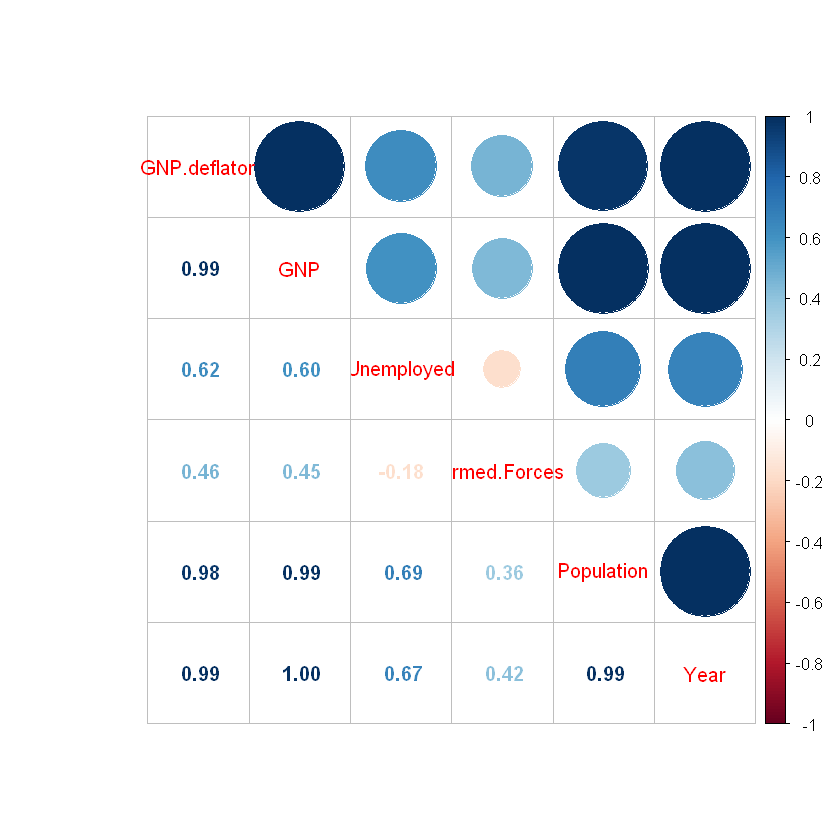
\includegraphics[scale=0.4]{output_8_1.png}
	\caption{相关系数图}
\end{figure}

统计分析:

此图中圆圈越大颜色越深说明相关系数越接近1,变量间的相关性越强。可以看出图中有较多的圆圈是大且色深的,说明
变量之间存在复共线性。

\section{第二问:主成分回归}

\subsection{将回归方程化为典则形式}

源代码:

\begin{lstlisting}[language=r,breaklines]
phi=eigen(t(X)%*%X)$vectors
gam=diag(eigen(t(X)%*%X)$values)
Z=X%*%phi
\end{lstlisting}

统计分析:

记线性回归模型为:

\begin{equation*}
	\begin{aligned}
		& y=\alpha_0 1_n+X\beta+e\\
		& e\sim (0,\sigma^2 I_n)\\
	\end{aligned}
\end{equation*}

则其典则形式为:

\begin{equation*}
	\begin{aligned}
		& y=\alpha_0 1_n+Z\alpha+e\\
		& e\sim (0,\sigma^2 I_n)\\
	\end{aligned}
\end{equation*}

其中$Z \triangleq X\phi$,\ $\alpha \triangleq \phi'\beta$,\ $X'X=\phi\Gamma\phi'$,
$\Gamma=diag(\lambda_1,\cdots,\lambda_p)$为$X'X$的特征值构成的对角阵,$\phi=(\phi_1,\cdots,\phi_p)$为对应的标准正交的
特征向量组成的列向量组。

这里使用eigen函数求出了特征值矩阵gam和特征向量矩阵phi,并由此求出了Z,相当于求出了回归方程的
典则形式。

\subsection{主成分个数选择}

源代码:

\begin{lstlisting}[language=r,breaklines]
(gam[1,1]/sum(diag(gam)))
((gam[1,1]+gam[2,2])/sum(diag(gam)))
((gam[1,1]+gam[2,2]+gam[3,3])/sum(diag(gam)))
\end{lstlisting}
out: 0.767229515961399\quad 0.963119599170923 \quad 0.997023827904495

\begin{lstlisting}[language=r,breaklines]
PCA=princomp(X)
summary(PCA,loadings=T)
screeplot(PCA,type="lines")
Z1=X%*%phi[,1:3]
\end{lstlisting}
\begin{figure}[htbp]
	\centering
	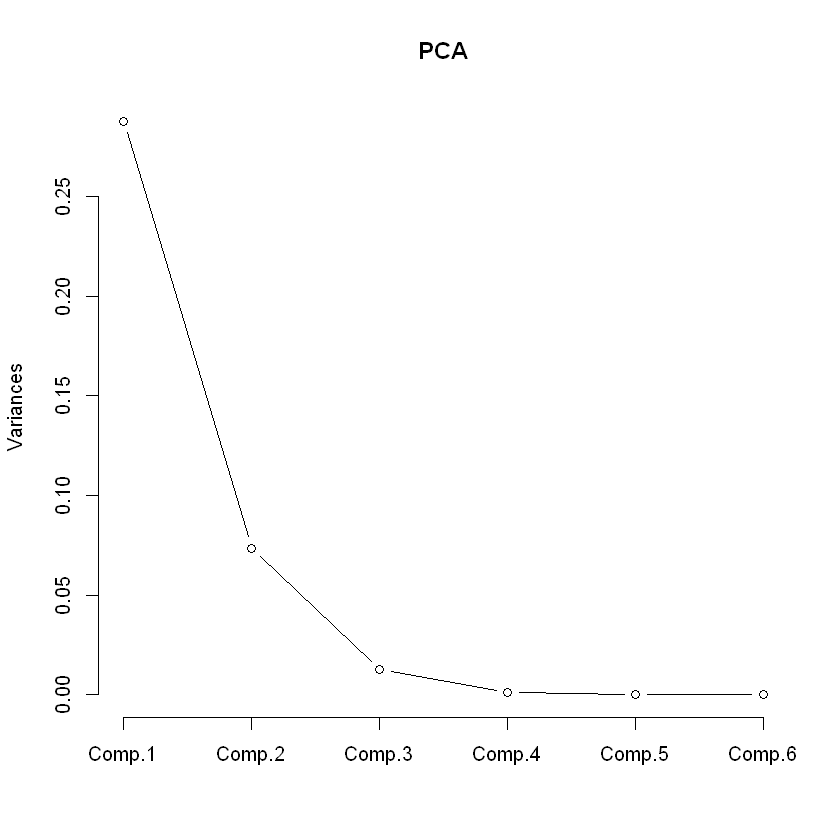
\includegraphics[scale=0.3]{output_18_1.png}
	\caption{碎石图}
\end{figure}

统计分析:

预先给定:当方差累计贡献率超过97\%时,停止选入主成分。这里计算了前两个(方差前二大的)主成分的方差累积贡献率,
在选入第三个主成分时就已经超过了97\%,于是选取三个主成分。从碎石图中也看出可以选取两个主成分。

记:$\phi_0=(\phi_1,\phi_2,\phi_3)$,$Z_1=X\phi_0$,$\alpha_1=\phi_0'\beta$
\subsubsection{讨论:如果选取两个主成分}
源代码:
\begin{lstlisting}[language=r,breaklines]
alph1=solve(t(Z1)%*%Z1)%*%t(Z1)%*%y
(beta1=phi[,1:2]%*%alph1)
\end{lstlisting}

out: 

\begin{figure}[htbp]
	\centering
	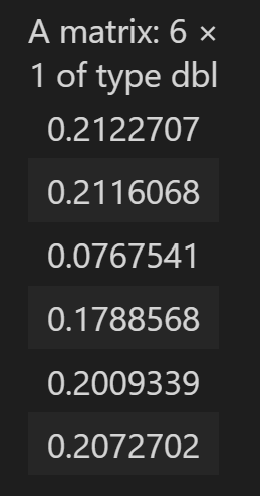
\includegraphics[scale=0.48]{jietu0.png}
	\caption{不合理的主成分回归结果}
\end{figure}

统计分析:

从上面的主成分回归结果可以看出,$\hat{\beta}$的分量的符号全为正,不符合变量的实际意义。
如第三个分量"Unemployed"和第四个分量"Armed.Forces"越大,因变量"Employed"应该越小,
故它们的系数的符号应该为负值,所以这个估计不符合实际意义。

\subsection{求主成分的最小二乘估计并代回原变量}

源代码:

\begin{lstlisting}[language=r,breaklines]
(alph0=mean(y))
alph1=solve(t(Z1)%*%Z1)%*%t(Z1)%*%y
beta1=phi[,1:3]%*%alph1
\end{lstlisting}
out: -4.92227786308419e-16


\begin{lstlisting}[language=r,breaklines]
inter=ymean-ysd*t(beta2)%*%(as.vector(xmean/xsd))
\end{lstlisting}
out: -358.7128

\begin{lstlisting}[language=r,breaklines]
betaz=ysd*(phi[,1:3]%*%alph2)/as.vector(xsd)
\end{lstlisting}
out: 0.094787894,0.012674214,-0.011614913,-0.005987296,0.153862145,0.202957527


\begin{lstlisting}[language=r,breaklines]
oldX%*%betaz+rep(inter,16)-oldY
\end{lstlisting}

out:
\begin{figure}[htbp]
	\centering
	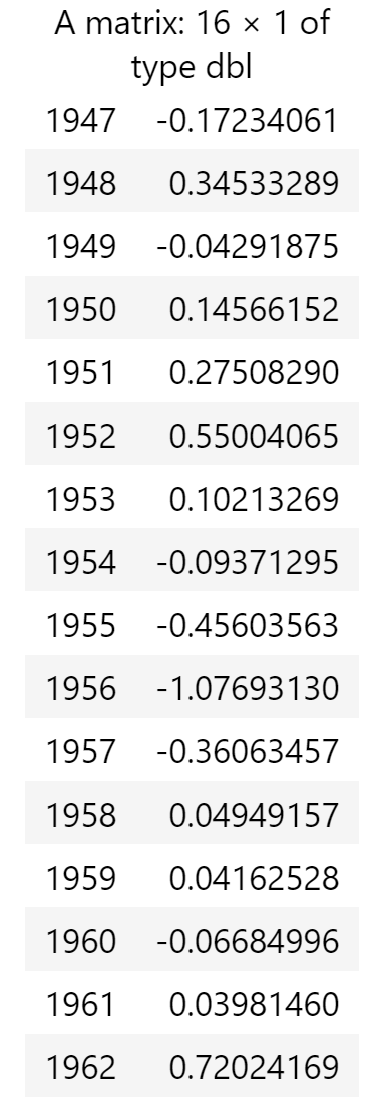
\includegraphics[scale=0.4]{jietu3.png}
	\caption{主成分回归残差}
\end{figure}

统计分析:

将剩余的主成分对y做最小二乘回归:
$$\hat{\alpha_0}=\bar{y}$$
$$\hat{\alpha_1}=(Z_1'Z_1)Z_1'y$$

再返回到原来的自变量,得到$\beta$的最小二乘回归:
$$\hat{\beta}=\phi_0\hat{\alpha_1}\triangleq (\hat{\beta}_1,\cdots,\hat{\beta}_6)$$

由于做过中心标准化,下面将方程还原至中心标准化之前的变量,仍用$x_1,\cdots,x_6$表示。

$$\frac{\hat{y}-\bar{y}}{s_y}=\sum_{i=1}^{6}\hat{\beta}_i \frac{x_i-\bar{x}_i}{s_i}$$

即为:

$$\hat{y}=\bar{y}-s_y \sum_{i=1}^{6} \hat{\beta}_i \frac{\bar{x}_i}{s_i} + s_y \sum_{i=1}^{6} \frac{\hat{\beta}_i}{s_i} x_i$$
代入数据计算得到如下的主成分回归方程:
$$\hat{y}=-358.7128+0.0948x_1+0.0127x_2-0.0116x_3-0.006x_4+0.1539x_5+0.2030x_6$$

计算残差向量如图4所示,可见残差向量各分量均较小,拟合效果较好。
\section{第三问:岭回归}

源代码:

\begin{lstlisting}[language=r,breaklines]
betahat <- function(k){
    return (solve(t(X)%*%X+k*diag(6))%*%t(X)%*%y)
}
\end{lstlisting}

统计分析:

这里是定义了岭回归估计量$\hat{\beta}(k)=(X'X+kI_p)^{-1}X'y\triangleq (\hat{\beta}_1 (k),\cdots,\hat{\beta}_6 (k))$。其中,
k被称为岭参数。下面用三种方法来估计岭参数:

\subsection{岭迹法}

源代码:

\begin{lstlisting}[language=r,breaklines]
dd<- as.data.frame(t(rbind(seq(0,0.03,0.00001),sapply(seq(0,0.03,0.00001),betahat))))
write.csv(dd,"dd.csv")
\end{lstlisting}
\begin{lstlisting}[language=python,breaklines]
df=pd.read_csv("dd.csv")
df.iloc[:,1:].plot(x="V1",legend=False)
import matplotlib.pyplot as plt
plt.savefig("lingji.png")
\end{lstlisting}
out: 

\begin{figure}[htbp]
	\centering
	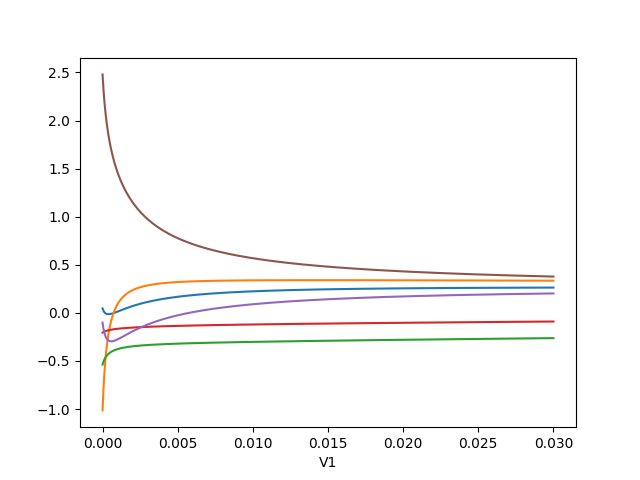
\includegraphics[scale=0.45]{lingji.png}
	\caption{岭迹图}
\end{figure}

\begin{lstlisting}[language=r,breaklines]
(inter1=ymean-ysd*t(betahat(0.02))%*%(as.vector(xmean/xsd)))
\end{lstlisting}
out: -575.2279

\begin{lstlisting}[language=r,breaklines]
(betal1=ysd*(betahat(0.02))/as.vector(xsd))
\end{lstlisting}

out: 0.0831301699985482, 0.0119777673450668,-0.0105029944945249,

-0.00518425678976126,0.0865205092723138,0.318236949235663

\begin{lstlisting}[language=r,breaklines]
oldX%*%betal1+rep(inter1,16)-oldY
\end{lstlisting}

out:
\begin{figure}[htbp]
	\centering
	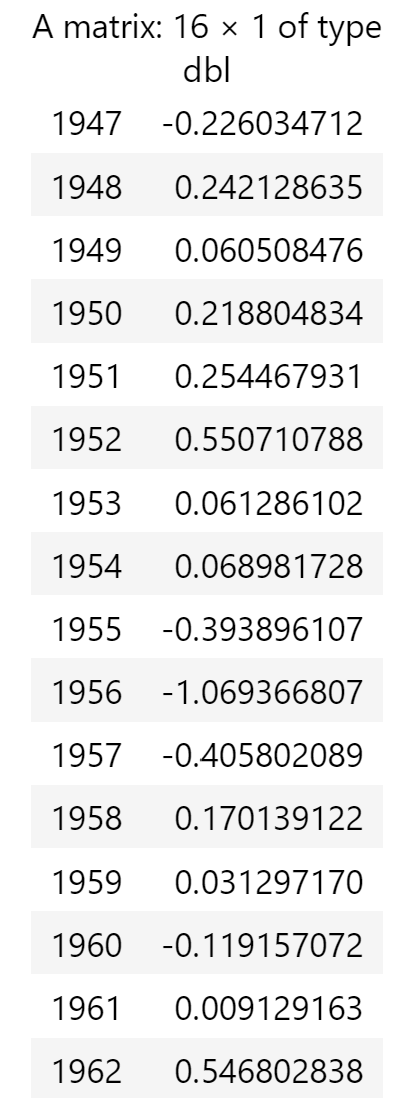
\includegraphics[scale=0.5]{jietu1.png}
	\caption{岭估计(k=0.020)的残差}
\end{figure}

统计分析:

岭迹法中岭参数的选取标准为:
\begin{itemize}
	\item 使各个回归系数的岭估计大体上稳定
	\item 各个回归系数的岭估计值的符号比较合理
	\item 残差平方和不要上升太多
\end{itemize}

于是岭参数k不宜太大或太小,故我们选取了k=0.020。

由于做过中心标准化,下面将方程还原至中心标准化之前的变量,仍用$x_1,\cdots,x_6$表示。

$$\frac{\hat{y}-\bar{y}}{s_y}=\sum_{i=1}^{6}\hat{\beta}_i (0.02) \frac{x_i-\bar{x}_i}{s_i}$$

即为:

$$\hat{y}=\bar{y}-s_y \sum_{i=1}^{6} \hat{\beta}_i (0.02) \frac{\bar{x}_i}{s_i} + s_y \sum_{i=1}^{6} \frac{\hat{\beta}_i (0.02)}{s_i} x_i$$
代入数据计算得到如下的岭回归方程:
$$\hat{y}=-575.2279+0.0831x_1+0.0120x_2-0.0105x_3--0.0052x_4+0.0865x_5+0.3182x_6$$

计算残差向量如图6所示,可见残差向量各分量均较小,拟合效果较好。

\subsection{方差扩大因子法}

源代码:

\begin{lstlisting}[language=r,breaklines]
chat <- function(k){
	return (max(diag(solve(t(Z)%*%Z+diag(k,6))%*%t(Z)%*%(Z)%*%solve(t(Z)%*%Z+diag(k,6)))))
}
plot(seq(0.01,0.2,0.001),lapply(seq(0.01,0.2,0.001),chat))
abline(h=10,v=0.024)
\end{lstlisting}

out: 

\begin{figure}[htbp]
	\centering
	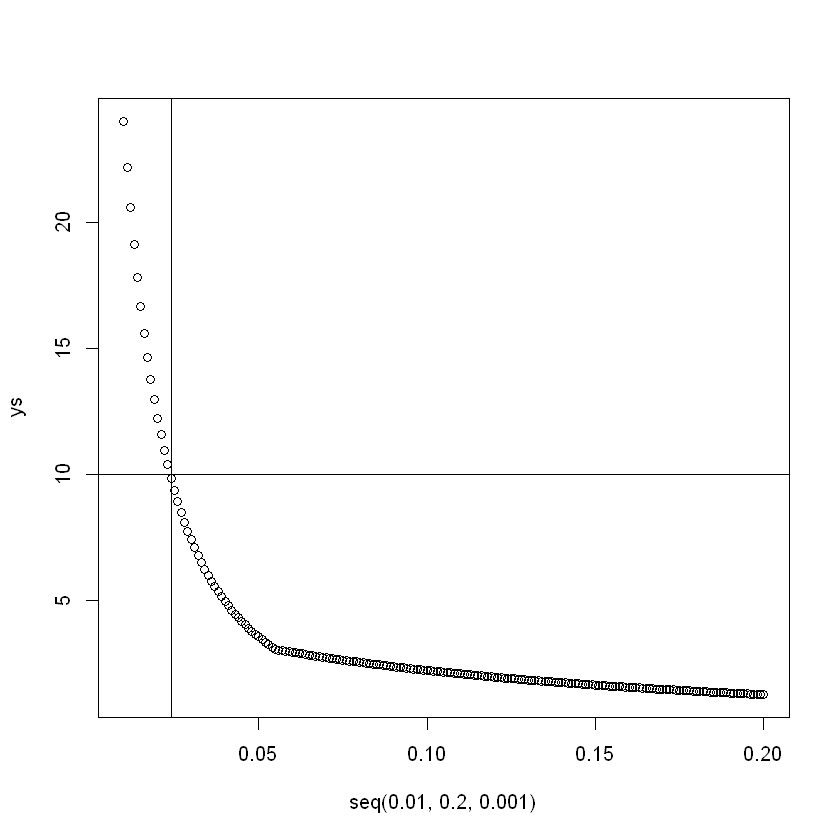
\includegraphics[scale=0.46]{output_31_0.png}
	\caption{方差扩大因子图}
\end{figure}

\begin{lstlisting}[language=r,breaklines]
(inter2=ymean-ysd*t(betahat(0.024))%*%(as.vector(xmean/xsd)))
\end{lstlisting}
out: -538.6605

\begin{lstlisting}[language=r,breaklines]
(betal2=ysd*(betahat(0.024))/as.vector(xsd))
\end{lstlisting}

out: 0.0845302428494129,0.0119224614765523,-0.0102338477540399,

-0.00490294566821215,0.0942791278588035,0.298918108195488
\begin{lstlisting}[language=r,breaklines]
oldX%*%betal2+rep(inter2,16)-oldY
\end{lstlisting}

out: 

\begin{figure}[htbp]
	\centering
	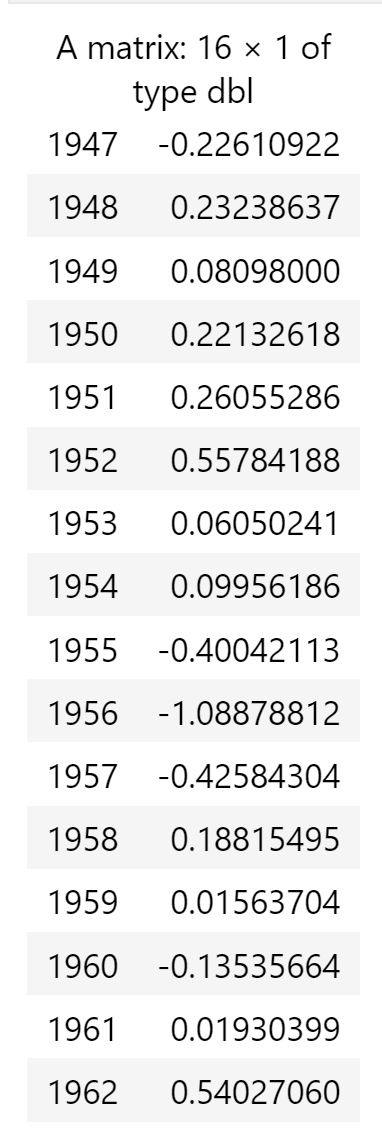
\includegraphics[scale=0.5]{jietu2.png}
	\caption{岭估计(k=0.024)的残差}
\end{figure}

统计分析:

根据前面给出的方差扩大因子的定义,可以知道矩阵$c(k)=(X'X+kI)^{-1}X'X(X'X+kI)^{-1}$的
对角元$c_{ii}(k)$为岭估计的方差扩大因子。原则为:选择使得所有$c_{ii}(k)$均不超过10的k值。
上面图像的y轴代表的是当前k下$c_{ii}(k)$中的最大值,当$c_{ii}(k)$中的最大值都小于10时,则
所有$c_{ii}(k)$均不超过10。故选择k=0.024。

由于做过中心标准化,下面将方程还原至中心标准化之前的变量,仍用$x_1,\cdots,x_6$表示。

$$\frac{\hat{y}-\bar{y}}{s_y}=\sum_{i=1}^{6}\hat{\beta}_i (0.024) \frac{x_i-\bar{x}_i}{s_i}$$

即为:

$$\hat{y}=\bar{y}-s_y \sum_{i=1}^{6} \hat{\beta}_i (0.024) \frac{\bar{x}_i}{s_i} + s_y \sum_{i=1}^{6} \frac{\hat{\beta}_i (0.024)}{s_i} x_i$$
代入数据计算得到如下的岭回归方程:
$$\hat{y}=-538.6605+0.0845x_1+0.0119x_2-0.0102x_3-0.0049x_4+0.0943x_5+0.2989x_6$$

计算残差向量如图8所示,可见残差向量各分量均较小,拟合效果较好。


\end{document}